\section{Model Performance Metrics \& Evaluation of Results}

\subsection{Plain Models}

When examining the distribution of our dataset by the target variable, it is evident that the majority of the results are `no', followed by `maybe' and `yes'. This distribution can be confirmed in Table~\ref{tab:dataset_target_variable}.

\begin{table}[H]
    \centering
    \caption{Original dataset Target Variable Balance}
    \label{tab:dataset_target_variable}
    \begin{tabular}{p{2.5cm}cp{8.5cm}} \hline
     \textbf{Required Treatment} & \textbf{Size} & \textbf{Comment}
     \\ \hline\hline
      no & 841668 (80\%) & Patients with COVID 19 that does not
      required hospitalization. \\ 
      maybe & 117155 (11\%) & Patients with COVID 19 that required
      further analysis (Inconclusive by the data). \\ 
      yes & 89752 (9\%) & Patients with COVID 19 that requires 
      hospitalization.\\ \hline
    \end{tabular}
\end{table}

Due to the presence of an \emph{imbalanced target variable} in our
dataset, we must exercise caution when analyzing the performance 
and reliability of our model. The predominance of the `no' class
could introduce a bias, skewing predictions toward this outcome.

Furthermore, it is crucial to monitor the model's performance 
regarding the minority classes, `maybe' and `yes', which are pivotal
to our predictive objectives. These outcomes are critical as they
relate directly to our goal of accurately identifying severe cases
of COVID-19, ensuring that these individuals receive hospital care
rather than being inappropriately sent home. Therefore, a thorough 
evaluation of the model's accuracy for these classes is essential
to avoid potentially grave errors in clinical decision-making.

So the most important metrics to analyze a Imbalanced Dataset
in a classification model are:
\begin{description}
    \item[Precision] Precision measures the positive predictions
    made\footnote{Off all the instances classified as positive, how
    many are positive?} (Equation~\ref{eqn:precision}). Precision
    is particularly important where the cost of a false positive is
    high;
    \item[Recall] On the other hand Recall measures the model's 
    ability to identify all positives in the dataset\footnote{
    Off all the actual positives, how many were identified 
    correctly by the model?}. This metric is specially important
    in our case because In a medical diagnosis for COVID-19 we 
    need
    to reduce the false negatives. This means reducing the risk of
    not treating patients that need. The Equation~\ref{eqn:recall}
    shows that
    there's a trade-off between precision and recall. Improving 
    the precision will reduce the recall and vice-versa;
    \item[AUC] AUC provides an aggregate performance across
    all possible classification thresholds. AUC needs to be closer
    to $1$ for a good classifier. Any value $\le 1$ is a worthless
    classifier with no better accuracy than a random chance.
\end{description}

\begin{equation}
\label{eqn:precision}
Precision = \frac{True Positives (TP)}{True Positives (TP) + False Positives (FP)}
\end{equation}

\begin{equation}
\label{eqn:recall}
Recall = \frac{True Positives (TP)}{True Positives (TP) + False Negatives (FN)}
\end{equation}

After following running the models we got the results presented
in the Table~\ref{tab:model_results}.

\begin{table}[H]
    \centering
    \caption{Evaluation Model Scores}
    \label{tab:model_results}
    \begin{tabular}{cccccc} \hline
     \textbf{Model} & \textbf{Recall} & \textbf{Prec} & \textbf{AUC} & \textbf{F1} & \textbf{CA} \\ \hline\hline
     Catboost       & 0.867 & 0.850 & 0.913 & 0.856 & 0.867 \\ 
     Neural Network & 0.866 & 0.848 & 0.912 & 0.855 & 0.866 \\ 
     Random Forest  & 0.857 & 0.840 & 0.886 & 0.847 & 0.857 \\ \hline
    \end{tabular}
\end{table}

We also have the confusion in the Figure~\ref{fig:confusion_matrix} and the Roc 
Curves for every output in Figure~\ref{fig:roc_curve}.

\begin{figure}[H]%
    \caption{Confusion Matrix Per Model}%
    \label{fig:confusion_matrix}%
    \centering
    \subfloat[\centering Catboost]{{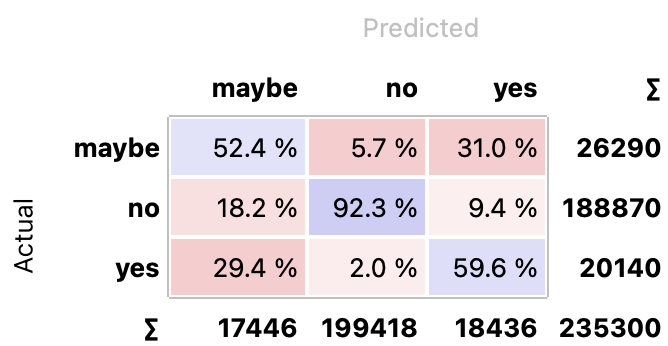
\includegraphics[width=0.45\textwidth]{img/evaluation/cm_gb.png} }}%
    \qquad
    \subfloat[\centering Neural Networks]{{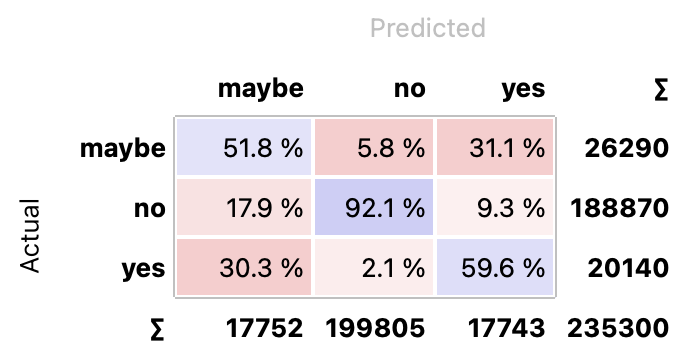
\includegraphics[width=0.45\textwidth]{img/evaluation/cm_nn.png} }}%
     \qquad
    \subfloat[\centering Random Forest]{{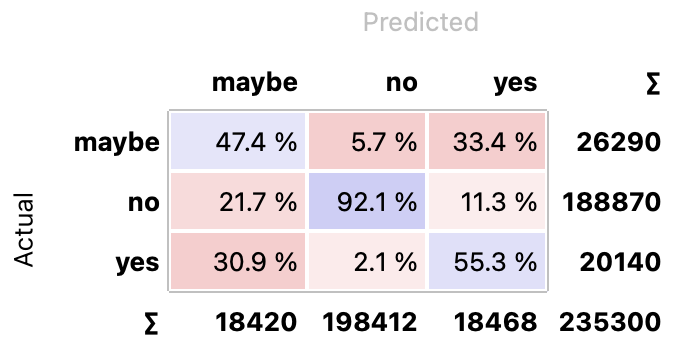
\includegraphics[width=0.45\textwidth]{img/evaluation/cm_rf.png} }}%
\end{figure}

\begin{figure}[H]%
    \caption{ROC Curves for the Outcomes}%
    \label{fig:roc_curve}%
    \centering
    \subfloat[\centering Yes]{{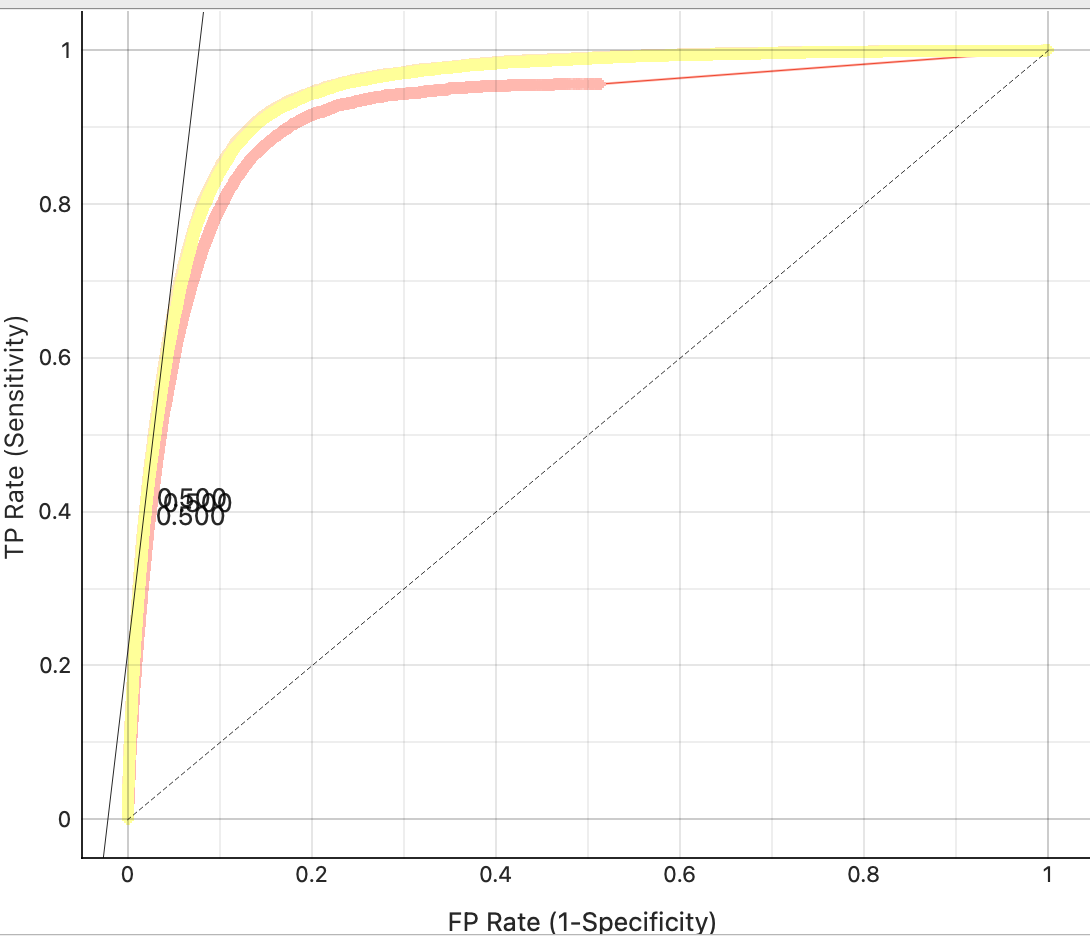
\includegraphics[width=0.45\textwidth]{img/evaluation/roc_yes.png} }}%
    \qquad
    \subfloat[\centering No]{{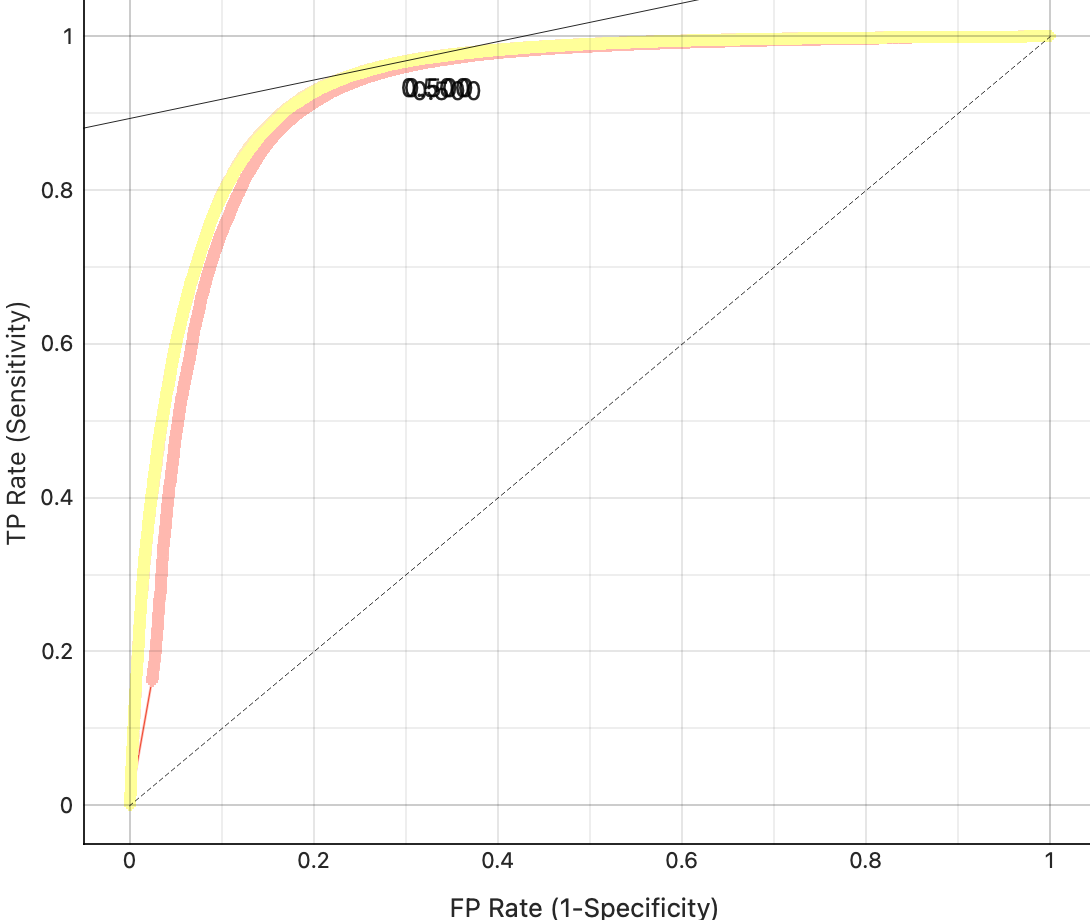
\includegraphics[width=0.45\textwidth]{img/evaluation/roc_no.png} }}%
     \qquad
    \subfloat[\centering Maybe]{{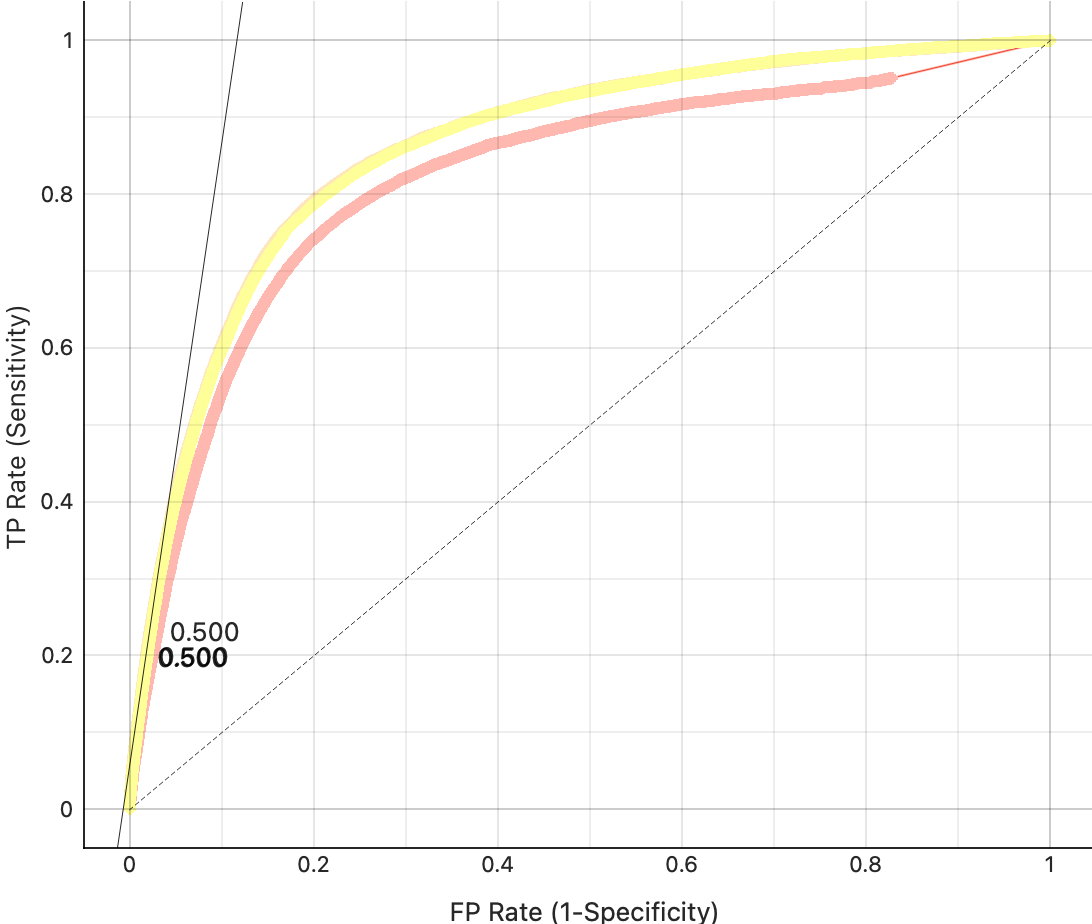
\includegraphics[width=0.45\textwidth]{img/evaluation/roc_maybe.png} }}%
\end{figure}

As anticipated, given that our dataset predominantly consists of categorical 
variables, the most effective classification model for this scenario is 
\emph{Catboost}. Unexpectedly, Neural Networks ranked second, outperforming
Random Forests, which came in last. The superior performance of
\emph{Neural Networks} over Random Forests could be attributed to the non-linear 
relationships among the features, or possibly because the Random Forest model 
became overfitted.

Regarding our results, it is apparent that predicting when a patient does not need 
hospitalization is both straightforward and accurate. We achieve a commendable 
accuracy rate of 90.7\% in this scenario, with only a 2.7\% error rate\footnote{Here, we only consider the `yes' value because `maybe' indicates a need for further analysis.}.

However, the same cannot be said for predicting the necessity of hospitalization.
Predicting whether a patient requires treatment proved to be challenging, with an
accuracy of only 61.1\% in confidently determining the need for hospitalization.
An additional 32.2\% of cases required further analysis, and unfortunately, 6.7\% of 
patients were incorrectly sent home. This 6.7\% represents a significant proportion 
of misclassified cases. To improve accuracy, the algorithm might benefit from 
training on a larger dataset of hospitalized patients. It's possible that even a 
dataset size of one million might not suffice, or perhaps the model requires 
additional features or data to enhance the reliability of these predictions.

As for predicting cases that fall into the `maybe' category, which as anticipated,
is the most challenging to predict, our model achieves less than 49.2\% accuracy.
On a positive note, 30.7\% of these cases were escalated to hospitalization, 
and 20.1\% were not, which suggests some level of effective triage. Since `maybe'
inherently implies the need for human intervention and further analysis, the 
implications of these predictions are not immediately dire. Nevertheless, similar 
to the `yes' predictions, enhancing model accuracy in this area would likely 
require more data for training.

\subsection{Stacked Feature Specific Models}
\label{subsec:stack}

Once we discovered the strengths and limitations of the standard models, we tested a 
number of custom stacked models. We want our stacked models to make conservative 
predictions, so they only send a patient home or straight to hospital if all sub-models 
agree. If any sub-model does not agree the patient will be sent for triage. The 
sub-models were trained on three specific feature sets, these were deliberately
chosen to make unanimous predictions harder and the stacked model safer.

The model returns `yes' when a patient should be treated in hospital and `no'
when the patient should recover at home. It returns `maybe' when a patient should
be triaged or when it cannot decide. The three way nature of this decision is very
important, saying `maybe' when a patient should recover at home is a true positive
result, likewise saying `maybe' when a patient should be treated in hospital is also 
a true positive. When evaluating the effectiveness of these models we should compare
them with whether the patient needs hospitalisation rather than the target variable
used to train the model. This results in an adjusted confusion matrix as seen in Table~\ref{tab:model_results_stacked}. We treat the home and hospital like two different 
questions and then measure the precision and recall for both. Given the nature of
the decision the model is making, saying `no' when the patient should be treated in
hospital has the worst outcome for the patient. As a results we want this value
to be as small as possible. A corollary of this is that we want the precision
for this decision to be as high as possible.

\begin{table}[ht]
    \centering
    \caption{Evaluation Scores for Stacked Models}
    \label{tab:model_results_stacked}
    \subcaption{All Models Stacked}
    \begin{tabular}{c|ccc}
                          & \textbf{maybe} & \textbf{no} & \textbf{yes} \\ \hline
        \textbf{home}     &          0.067 &       0.741 &         0.001 \\
        \textbf{hospital} &          0.134 &       0.041 &         0.016
    \end{tabular}
    \quad\qquad
    \begin{tabular}{cc}
        \textbf{Precision} & \textbf{Recall}  \\ \hline
            0.998 & 0.952  \\
            0.786 & 0.991
    \end{tabular}
    \bigskip
    \subcaption{Stacked Gradient Boosting (Catboost) with Neural Network}
    \begin{tabular}{c|ccc}
                          & \textbf{maybe} & \textbf{no} & \textbf{yes} \\ \hline
        \textbf{home}     &          0.041 &       0.764 &         0.004 \\
        \textbf{hospital} &          0.115 &       0.048 &         0.027
    \end{tabular}
    \quad\qquad
    \begin{tabular}{cc}
        \textbf{Precision} & \textbf{Recall}  \\ \hline
            0.995 & 0.943  \\
            0.746 & 0.971
    \end{tabular}
    \bigskip
    \subcaption{Stacked Gradient Boosting (Catboost)}
    \begin{tabular}{c|ccc}
                          & \textbf{maybe} & \textbf{no} & \textbf{yes} \\ \hline
        \textbf{home}     &          0.039 &       0.765 &         0.004 \\
        \textbf{hospital} &          0.111 &       0.050 &         0.029
    \end{tabular}
    \quad\qquad
    \begin{tabular}{cc}
        \textbf{Precision} & \textbf{Recall}  \\ \hline
            0.993 & 0.941  \\
            0.736 & 0.963
    \end{tabular}
    \bigskip
    \subcaption{Stacked Random Forest with Neural Network}
    \begin{tabular}{c|ccc}
                          & \textbf{maybe} & \textbf{no} & \textbf{yes} \\ \hline
        \textbf{home}     &          0.049 &       0.756 &         0.004 \\
        \textbf{hospital} &          0.120 &       0.047 &         0.024
    \end{tabular}
    \quad\qquad
    \begin{tabular}{cc}
        \textbf{Precision} & \textbf{Recall}  \\ \hline
            0.995 & 0.945  \\
            0.754 & 0.975
    \end{tabular}
    \bigskip
    \subcaption{Stacked Random Forest}
    \begin{tabular}{c|ccc}
                          & \textbf{maybe} & \textbf{no} & \textbf{yes} \\ \hline
        \textbf{home}     &          0.046 &       0.758 &         0.005 \\
        \textbf{hospital} &          0.115 &       0.051 &         0.025
    \end{tabular}
    \quad\qquad
    \begin{tabular}{cc}
        \textbf{Precision} & \textbf{Recall}  \\ \hline
            0.994 & 0.941  \\
            0.735 & 0.967
    \end{tabular}
\end{table}

The first observation is that the Stacked Gradient Boosting performs better than 
Stacked Random Forest. This is to be expected given the categorical nature of
the data.

Secondly including the Neural Network in the stack improves both the Stacked 
Gradient Boosting and the Stacked Random Forest. It reduced the false positives
for Stacked Gradient Boosting from 5\% to 4.8\%. And it reduced the false 
positives for Stacked Random Forest from 5.1\% to 4.7\%. This indicates the
Neural Network has found other characteristics in the data not found in the other
models. When this is included in our conservative stacking algorithm it reduces the 
`yes' and `no' results in favour of more `maybe's'. 

Thirdly it is interesting that the Stacked Random Forest with Neural Network
performs better than Stacked Gradient Boosting (Catboost) with Neural Network.
This shows that the results generated from Gradient Boosting are close to the 
results generated by the Neural Network

Finally when we stack all models together we see a much larger improvement. The
false positives are 4.1\% and the precision is 0.786. Ideally the precision should
be higher for a medical application, however there are some times when this could be
acceptable as discussed in Section~\ref{apply_model}.

\subsection{Applying the Model}
\label{apply_model}

The goal of applying this model is to reduce contact between patients and frontline
health professionals. Ordinarily they would triage all patients however since COVID-19
is so infectious and the Personal Protective Equipment (PPE) required to protect staff
is in short supply in the pandemic, the health system must protect its staff and conserve
PPE to remain functional. This is an emergency situation and not a normal application of
a medical model.

Compare the flow of patients in Figure~\ref{fig:triage_process}, with the normal triage process
100\% of patients need to be triaged, when the patients are screened first by the model
only 20\% of patients have to be triaged. We can clearly see 4\% of the population are sent home
in error. Not all patents required the same level of treatment in hospital, when we cross
reference the 4\% with the sickest patients requiring ICU we see this grave error is only
0.8\% of the population. Hopefully any patients sent home by the screening process would be 
able to return to the hospital as their symptoms worsen.

When we examine the patients sent straight to hospital we see this accounts for 1.7\% of 
the population, included in that is 0.1\% who do not require hospitalisation. Given the
population routed straight to hospital is so small, it probably makes sense to include 
this group in the triage process. As it would only change the triage reduction from 80\% to
78\%.

Based on this evaluation we could only recommend applying this model and the screening process
in the most grave emergency situation like the COVID-19 pandemic, where frontline health
professionals were risking their lives to treat patients and their infection rates risked
the efficacy of the health system as a whole.

\begin{figure}[H]
\caption{Triage Process}
\label{fig:triage_process}
\centering
\begin{subfigure}{.8\textwidth}
  \centering
  \caption{Normal Triage Process }
  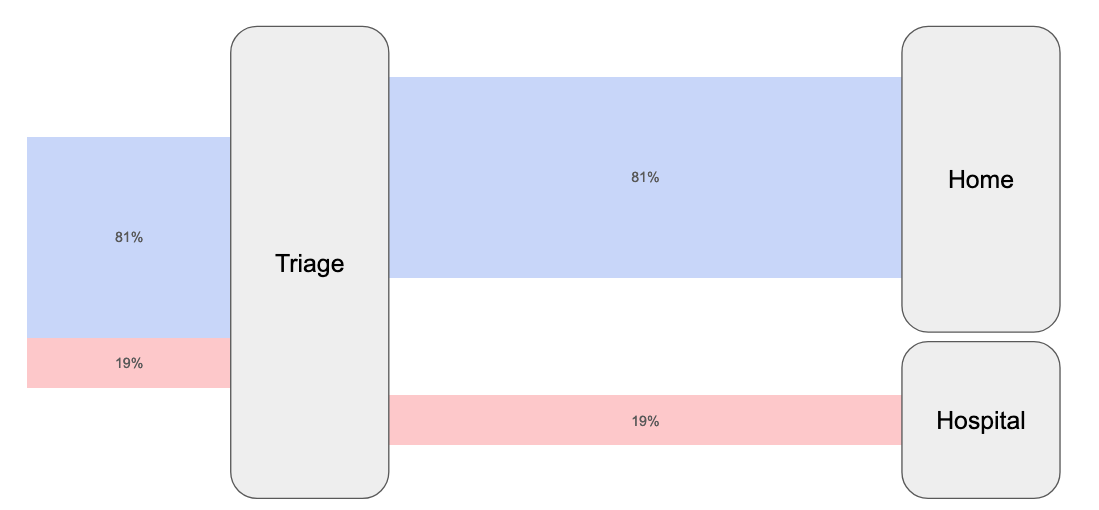
\includegraphics[width=\linewidth]{img/evaluation/triage_before.png}
\end{subfigure}% 
\qquad
\begin{subfigure}{.8\textwidth}
  \centering
  \caption{Triage Process with our Model}
  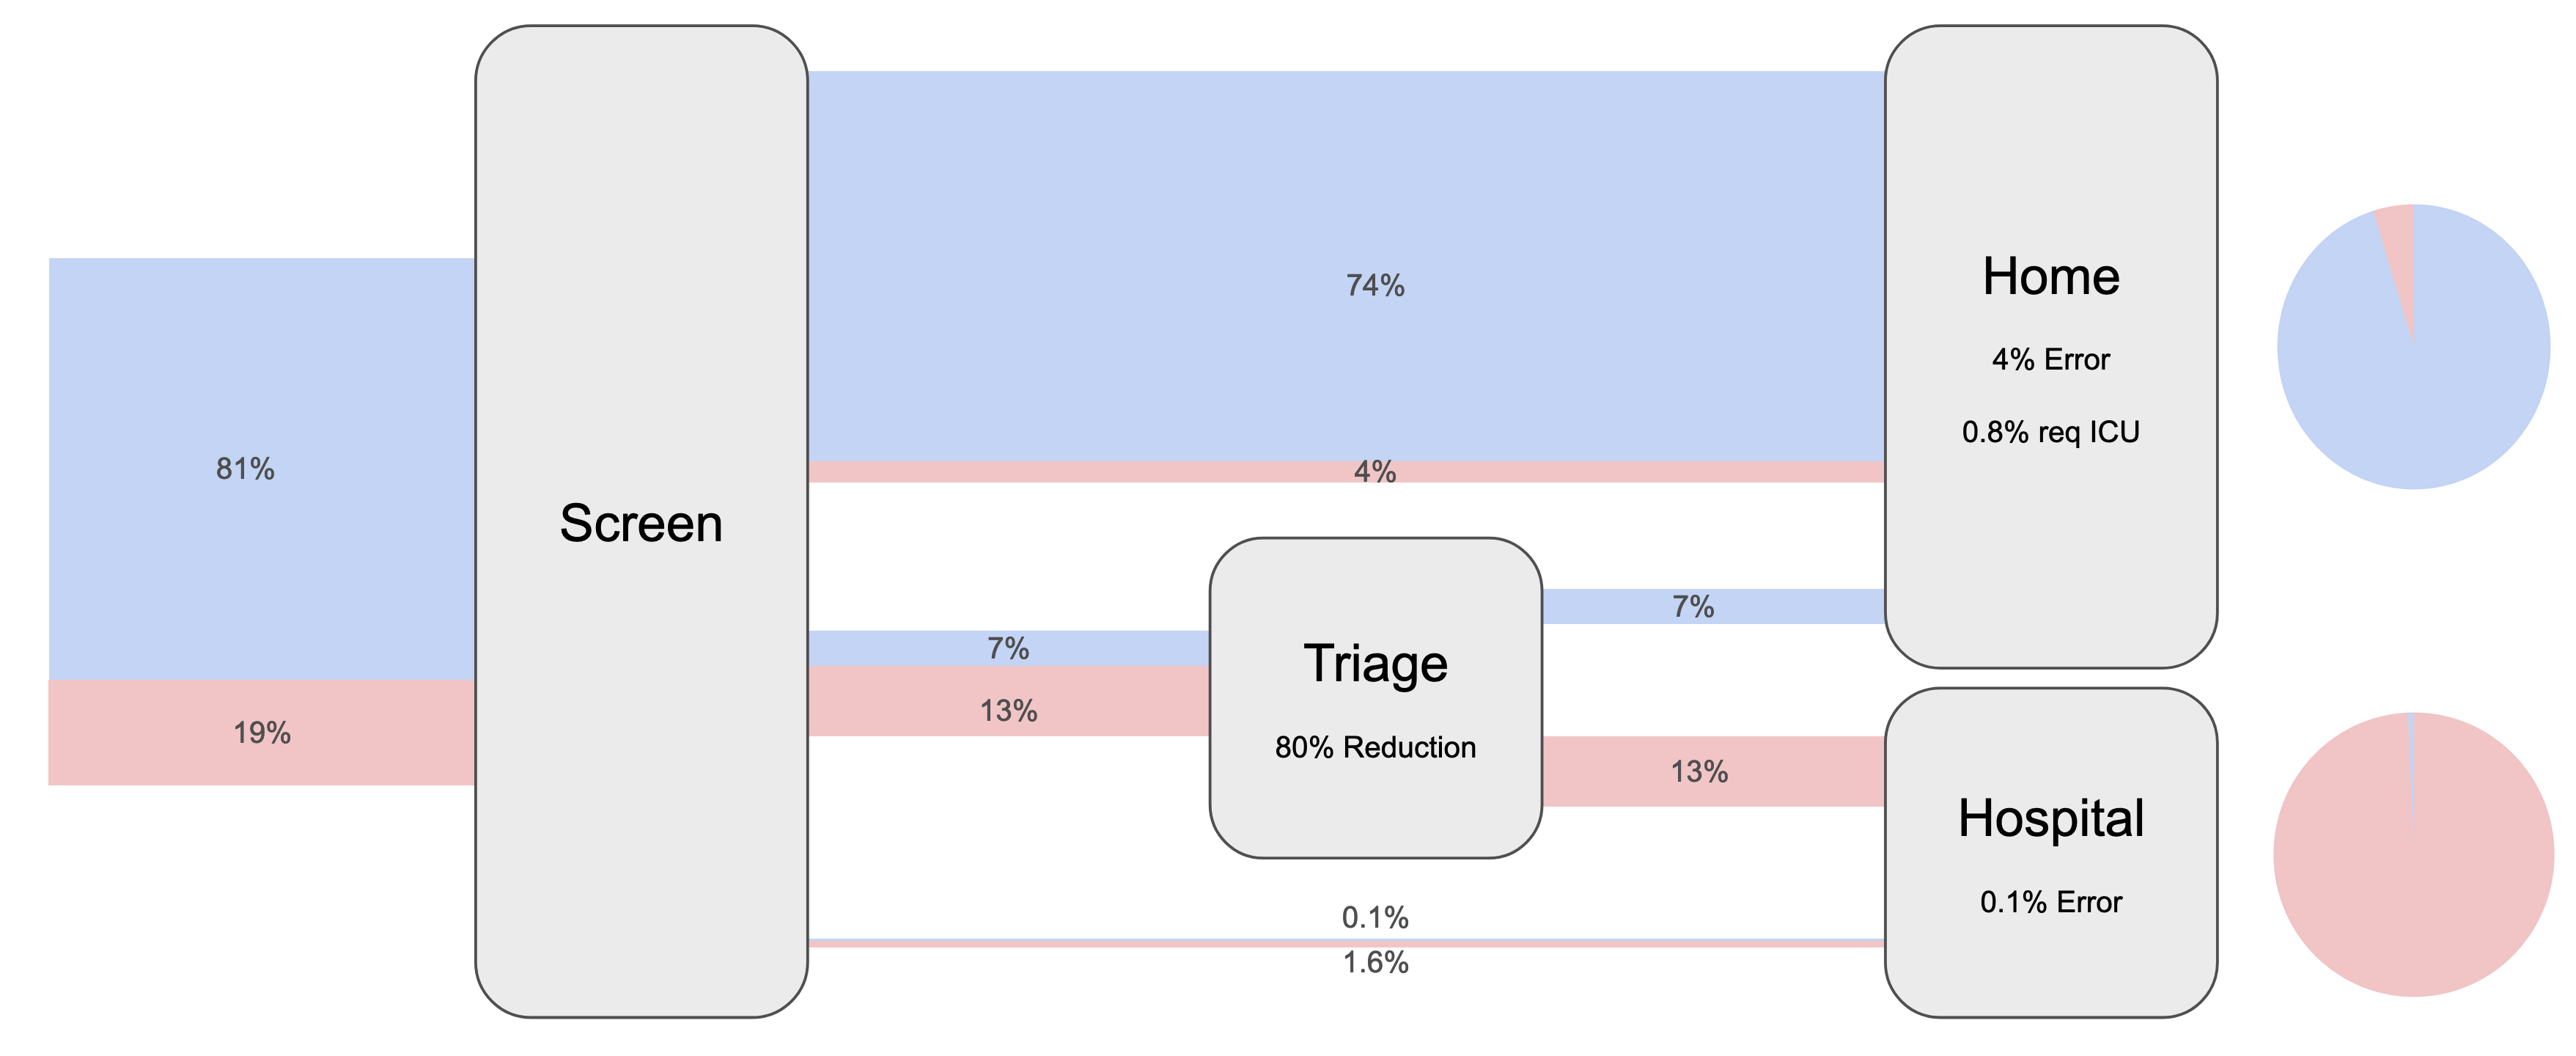
\includegraphics[width=\linewidth]{img/evaluation/triage_after.png}
\end{subfigure}
\end{figure}
